\section{详细设计}

本章节将描述云盘系统的详细设计,包括数据表结构和算法流程。

\subsection{数据表结构}

本章节将描述云盘系统的数据表结构。

\begin{table}[!ht]
    \centering
    \caption{用户表}
    \label{table:user}
    {
        \begin{tabularx}{1.0\textwidth}{|p{1.5cm}|p{2cm}|p{0.5cm}|p{1cm}|X|}
            
            \hline
            名称 & 类型 & 必填 & 特殊 & 描述  \\ 
            \hline
            用户ID & bigint & 是 & 主键 & 用户的唯一标识符。  \\ 
            用户名 & varchar(20) & 是 & - & 用户的名称  \\ 
            密码 & varchar(20) & 是 & - & 用户的密码  \\ 
            手机号 & varchar(15) & 是 & - & 用户的手机号(包括区号)  \\ 
            电子邮箱 & varchar(100) & 否 & - & 用户的电子邮箱  \\ 
            生日 & date & 否 & - & 用户的生日,包括年-月-日  \\ 
            角色 & short & 是 & - & 用户的角色,0表示普通用户,1表示管理员用户  \\ 
            \hline
        \end{tabularx}
    }
\end{table}

用户表结构如表\ref{table:user}所示,用户表中包含唯一标识符、用户名、密码,以及手机号、电子邮箱等描述信息。

\begin{table}[H]
    \centering
    \caption{文件表}
    \label{table:file}
    {
        \begin{tabularx}{1.0\textwidth}{|p{1.5cm}|p{2cm}|p{0.5cm}|p{1cm}|X|}
            \hline
            名称 & 类型 & 必填 & 特殊 & 描述  \\ 
            \hline
            文件ID & bigint & 是 & 主键 & 文件的唯一标识符  \\ 
            文件名 & varchar(100) & 是 & - & 文件的名称  \\ 
            文件类型 & varchar(20) & 是 & - & 文件类型,即后缀名  \\ 
            文件大小 & long & 是 & - & 文件大小,以KB为单位  \\ 
            hash值 & char(64) & 是 & - & 哈希值,用于检测文件已经存在  \\ 
            创建时间 & datetime & 是 & - & 文件创建的时间  \\ 
            本地路径 & varchar(200) & 是 & - & 存储在本地文件系统中的路径或对象存储的key  \\ 
            所属用户ID & bigint & 是 & 外键 & 所属用户的唯一标识符  \\ 
            \hline
        \end{tabularx}
    }
\end{table}

文件表结构如表\ref{table:file}所示,文件表中包含唯一标识符、文件名、类型、大小、hash值、创建时间、本地路径和所属用户ID的外键信息。

\begin{table}[H]
    \centering
    \caption{共享表}
    \label{table:share}
    {
        \begin{tabularx}{1.0\textwidth}{|p{1.5cm}|p{2cm}|p{0.5cm}|p{1cm}|X|}
            \hline
            名称 & 类型 & 必填 & 特殊 & 描述  \\ 
            \hline
            共享ID & bigint & 是 & 主键 & 分享的唯一标识符  \\ 
            属性 & short & 是 & - & 共享属性,0表示私人,1表示公共  \\ 
            密码 & varchar(8) & 否 & - & 分享链接的密码,如果有  \\ 
            截止时间 & datetime & 是 & - & 分享链接的有效期限  \\ 
            共享文件ID & bigint & 是 & 外键 & 共享文件的唯一标识符  \\ 
            接收用户ID & bigint & 否 & 外键 & 接收用户的唯一标识符,如果有  \\ 
            \hline
        \end{tabularx}
    }
\end{table}

共享表结构如表\ref{table:share}所示,共享表中包含唯一标识符、属性、密码、截止时间和文件ID、用户ID的外键信息。

\begin{figure}[H]
    \centering
    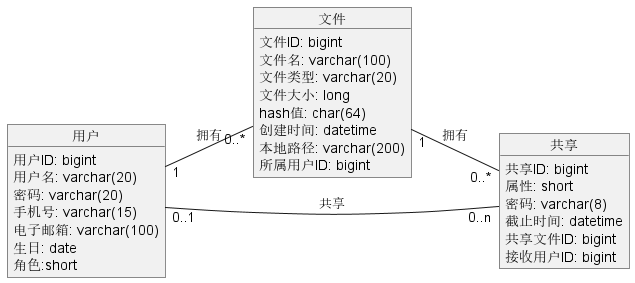
\includegraphics[scale=0.5]{examples/数据表结构图.png}
    \caption{数据表结构}
    \label{fig:table}
\end{figure}

数据表结构和关系如图\ref{fig:table}所示,其中用户可以拥有0至多个文件,一个文件只能属于一个用户,如果不同用户拥有的文件完整相同,将为其创建链接。一个共享链接只能指定一个文件,当模式为私人时,该共享只属于一个用户;否则,该文件属于所有公共用户。

\subsection{算法流程}

本章节将描述详细一些主要部分的算法流程。

\subsubsection{登录流程}

\begin{figure}[H]
    \centering
    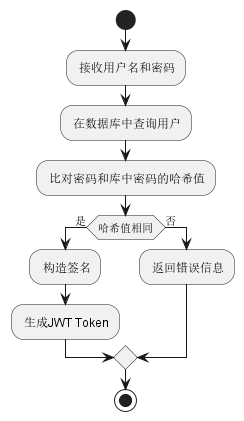
\includegraphics[scale=0.8]{examples/登录流程.png}
    \caption{登录流程}
    \label{fig:login}
\end{figure}

登录流程如图\ref{fig:login}所示,图中展示了一些细节:
\begin{itemize}
    \item 密码不能采用明文保存,而是采用MD5/SHA256等哈希算法加密后保存,之后在比对密码时也需要比对其哈希值,避免密码原文被泄露。
    \item 在比对通过后,将返回一个JWT Token,该token不需要在服务端存储,而是可以直接将一些用户信息,如盐、用户名、过期时间等信息写入并加密。当服务器收到一个token后,会尝试进行解码,只有解码成功才能拿到该用户的操作权限。
\end{itemize}

\subsubsection{文件上传流程}

\begin{figure}[H]
    \centering
    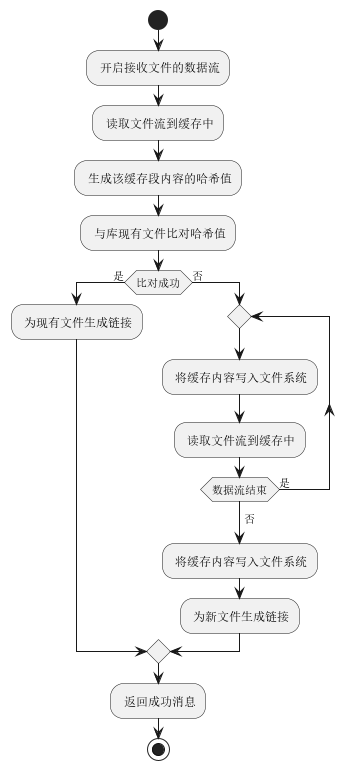
\includegraphics[scale=0.65]{examples/上传流程.png}
    \caption{上传流程}
    \label{fig:upload}
\end{figure}

文件上传流程如图\ref{fig:upload}所示,图中展示了一些细节:
\begin{itemize}
    \item 文件上传时首先会进行比对,具体来说,当读到文件的第一个数据流之后,就将其哈希值与库中保存的哈希值进行比对。如果有相同的值,则视为该文件已经存在,此时只需要对现有文件生成链接,避免文件的重复上传。
    \item 当文件不存在时,才需要写入文件系统并持续接收数据流直到关闭。
\end{itemize}
